\documentclass[11pt]{article}
\usepackage{geometry}
\usepackage{graphicx}
\usepackage{enumitem}
\usepackage{float}
\usepackage{amsmath}
\usepackage{multicol}
\usepackage{cancel}

\geometry{a4paper, top=0.5in, bottom=0.5in, right=0.75in, left=0.75in}

\title{Lecture 4}
\author{}
\date{}

\begin{document}

\maketitle

\section{Introduction}
\begin{itemize}
    \item From last lecture, the gain coefficient ($\gamma$) is given by: $\gamma = \sigma (N_2-N_1)$, so amplification is possible if $N_2 > N_1$.
    \item However, the number of atoms in each level follows the Boltzmann distribution, where the number of atoms decreases significantly with increasing energy level.
    \item Traditionally $N_2 << N_1$, so we have to do population inversion (pumping) to achieve amplification.
\end{itemize}

\section{4-Level Laser}
\begin{itemize}
    \item This model focuses on $E_2$ and $E_1$ levels as well as the ground level ($E_0$), and reduces all upper level into a single level ($E_3$).
    \item We want to pump atoms to $E_2$ only, but this is not possible because the input light is a spectrum (not a specific $\lambda$), which can excite atoms from $E_0$ to $E_1$ or $E_3$.
    \item To reduce the effect of pumping atoms from $E_0$ to $E_3$, we use a material with a very small lifetime for $E_3$, so that the atoms quickly drop to $E_2$.
    \item The lifetime of $E_2$ should be long enough to allow amplification.
\end{itemize}
\begin{center}
    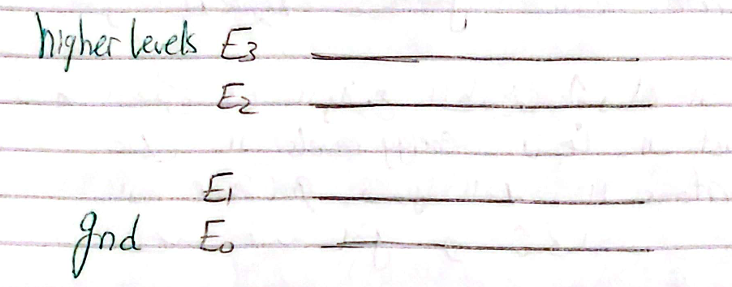
\includegraphics[scale=0.6]{1.png}
\end{center}
\subsection{Rate Equations during Pumping}
\begin{itemize}
    \item Note that the following equations takes into account only the spontaneous emission since the input light is for pumping not the signal that will be amplified.
    \item We check what influences the number of atoms in each level:
\end{itemize}

\begin{center}
    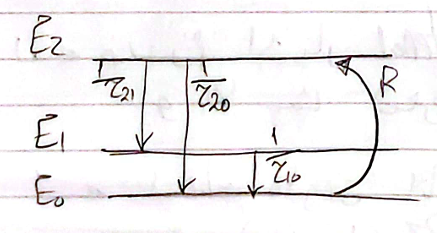
\includegraphics[scale=1]{2.png}
\end{center}
\begin{align*}
    \frac{dN_2}{dt} &= R - \frac{N_2}{\tau_{2}}
\end{align*}
where $R$ is the pumping rate and $\frac{1}{\tau_{2}} = \frac{1}{\tau_{21}} + \frac{1}{\tau_{20}}$ 
\begin{align*}
    \frac{dN_1}{dt} &= \frac{N_2}{\tau_{21}} - \frac{N_1}{\tau_{10}}
\end{align*}
Assume steady state, so $\frac{d}{dt} = 0$:
\begin{align}
    0 &= R - \frac{N_2}{\tau_{2}} \Rightarrow N_2 = R \tau_2 \\
    0 &= \frac{N_2}{\tau_{21}} - \frac{N_1}{\tau_{10}} \Rightarrow N_2 \tau_{10} = N_1 \tau_{21}
\end{align}
Substitute (1) into (2):
\begin{align}
    R \tau_2 \tau_{10} = N_1 \tau_{21} \Rightarrow N_1 = R \tau_2 \frac{\tau_{10}}{\tau_{21}}
\end{align}
(1) - (3):
\begin{align*}
    N_o = N_2 - N_1 = R \tau_2 \left(1 - \frac{\tau_{10}}{\tau_{21}}\right)
\end{align*}
where $N_o = N_2 - N_1$ when there is no input signal (just pumping). The correspoding gain coefficient is:
\begin{align*}
    \gamma_o = \sigma N_o
\end{align*}
To get population inversion, $\tau_{10} < \tau_{21}$, because we want the atoms to stay in $E_2$ longer than $E_1$.

\subsection{Rate Equations during Amplification}
\begin{itemize}
    \item To get frequency ($\nu = \frac{\Delta E}{h}$), the signal should have $\Delta E = E_2 - E_1$.
    \item Now we should consider the absorption and stimulated emission in addition to the spontaneous emission.
\end{itemize}
\begin{center}
    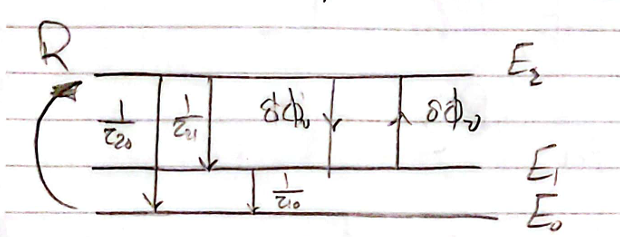
\includegraphics[scale=1]{3.png}
\end{center}
\begin{align*}
    \frac{dN_2}{dt} &= R - \frac{N_2}{\tau_{2}} - \sigma \phi_{\nu} N_2 + \sigma \phi_{\nu} N_1 \\
    \frac{dN_1}{dt} &= - \frac{N_1}{\tau_{10}} + \frac{N_2}{\tau_{21}} + \sigma \phi_{\nu} N_2 - \sigma \phi_{\nu} N_1 
\end{align*}
Assume steady state, so $\frac{d}{dt} = 0$:
\setcounter{equation}{0}
\begin{align}
    0 &= R - \frac{N_2}{\tau_{2}} - \sigma \phi_{\nu} N_2 + \sigma \phi_{\nu} N_1 \\
    0 &= - \frac{N_1}{\tau_{10}} + \frac{N_2}{\tau_{21}} + \sigma \phi_{\nu} N_2 - \sigma \phi_{\nu} N_1
\end{align}
From (1):
\begin{align}
    N_2 = R \tau_2 - \sigma \phi_{\nu}(N_2 - N_1) \tau_2
\end{align}
From (2):
\begin{align}
    N_1 - N_2 \frac{\tau_{10}}{\tau_{21}} = \sigma \phi_{\nu}(N_2 - N_1) \tau_{10}
\end{align}
We want $N_2 - N_2$, so (3) * $\left( 1- \frac{\tau_{10}}{\tau_{21}} \right)$ - (4):
\begin{align*}
    N_2 - \cancel{N_2 \frac{\tau_{10}}{\tau_{21}}} - N_1 + \cancel{N_2 \frac{\tau_{10}}{\tau_{21}}} = R \tau_2 \left( 1- \frac{\tau_{10}}{\tau_{21}} \right) - \sigma \phi_{\nu}\tau_2(N_2 - N_1) \left( 1- \frac{\tau_{10}}{\tau_{21}} \right) - \sigma \phi_{\nu} \tau_{10} (N_2 - N_1)
\end{align*}
So:
\begin{align*}
    N_2 - N_1 = -(N_2 - N_1) \sigma \phi_{\nu} \left[ \tau_{10} + \tau_2 \left( 1- \frac{\tau_{10}}{\tau_{21}} \right) \right] + R \tau_2 \left( 1- \frac{\tau_{10}}{\tau_{21}} \right)
\end{align*}
So:
\begin{align*}
    (N_2 - N_1) \left[ 1 + \sigma \phi_{\nu} \left[ \tau_{10} + \tau_2 \left( 1- \frac{\tau_{10}}{\tau_{21}} \right) \right] \right] = R \tau_2 \left( 1- \frac{\tau_{10}}{\tau_{21}} \right) = N_o
\end{align*}
Let $\tau_{10} + \tau_2 \left( 1- \frac{\tau_{10}}{\tau_{21}} \right) = \tau_s$:
\begin{align*}
    (N_2 - N_1) \left[ 1 + \sigma \phi_{\nu} \tau_s \right] = N_o
\end{align*}
Let $\sigma \tau_s = \frac{1}{\phi_s}$:
\begin{align*}
    (N_2 - N_1) \left[ 1 + \frac{\phi_{\nu}}{\phi_s} \right] = N_o
\end{align*}
So:
\begin{align*}
    N =  N_2 - N_1 = \frac{N_o}{1 + \frac{\phi_{\nu}}{\phi_s}}
\end{align*}
\textbf{Notes:}
\begin{itemize}
    \item $\frac{\phi_{\nu}}{\phi_s} = \frac{I_{\nu}}{I_s} = \frac{P_{\nu}}{P_s}$
    \item $\tau_2 < \tau_{21}$ since $\tau_2 = \tau_{21} || \tau_{20}$, so $\tau_s$ is positive.
    \item $\phi_s$ is the $\phi_{\nu}$ at which the population inversion is decreased by half ($N=\frac{N_o}{2}$).
    \item Note that as light flux density increases ($\phi_{\nu}$), the population inversion decreases.
    \item If the input signal was large, many atoms will transition from $E_2$ to $E_1$ at the begining, so as we move along the material, there will be a low number of atoms in $E_2$ to transition, so the gain will decrease.
    \item The source of amplification is the pumping, so efficiency is given by: $\eta = \frac{P_{\nu}}{P_{\text{pump}}}$
\end{itemize}
\begin{center}
    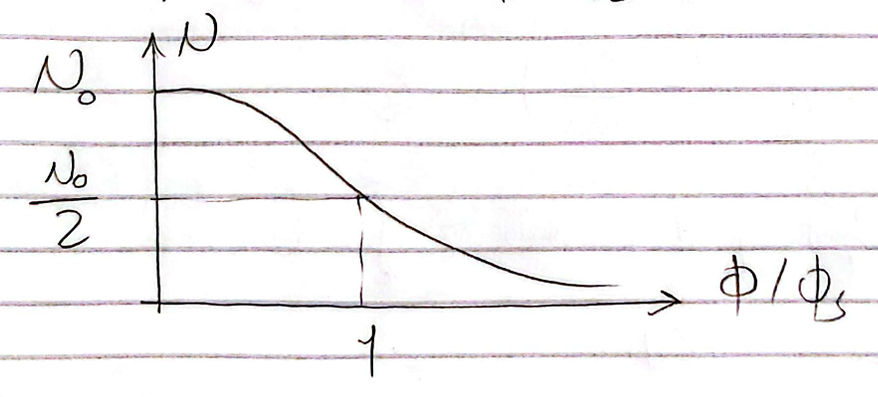
\includegraphics[scale=0.6]{4.png}
\end{center}

\subsection{Gain Saturation for Homogenously Broadened Medium}
If the gain is constant and does not depend on the input signal:
\begin{align*}
    \frac{d \phi}{dz} &= \gamma_o \phi \Rightarrow \phi(z) = \phi(0) e^{\gamma_o z} \\
    G_o &= \frac{\phi(L)}{\phi(0)} = e^{\gamma_o L}
\end{align*}
where $\gamma_o$ is unsaturated gain coefficient ($\frac{1}{m}$) and $G_o$ is the unsaturated gain (dimensionless). \\
If the gain depends on the input signal:
\begin{align*}
    \frac{d \phi}{dz} &= \frac{\gamma_o}{1 + \frac{\phi}{\phi_s}} \phi \\
    \gamma_o dz &= \frac{d \phi}{\phi} \left(1 + \frac{\phi}{\phi_s}\right)\\
    \gamma_o dz &= \frac{d \phi}{\phi} + \frac{d \phi}{\phi_s}
\end{align*}
Integrate:
\begin{align*}
    \int_{0}^{L} \gamma_o dz &= \int_{\phi_{\text{in}}}^{\phi_{\text{out}}} \frac{d \phi}{\phi} + \int_{\phi_{\text{in}}}^{\phi_{\text{out}}} \frac{d \phi}{\phi_s} \\
    \gamma_o L &= \ln \left( \frac{\phi_{\text{out}}}{\phi_{\text{in}}} \right) + \frac{1}{\phi_s} (\phi_{\text{out}} - \phi_{\text{in}}) \\
    \gamma_o L &= \ln \left( \frac{\phi_{\text{out}}}{\phi_{\text{in}}} \right) + \frac{\phi_{\text{in}}}{\phi_s} \left( \frac{\phi_{\text{out}}}{\phi_{\text{in}}} - 1\right) \\
\end{align*}
Let $\frac{\phi_{\text{out}}}{\phi_{\text{in}}} = G$, and from $ G_o = e^{\gamma_o L} \Rightarrow \ln G_o = \gamma_o L $:
\begin{align*}
    \gamma_o L&= \ln G + \frac{\phi_{\text{in}}}{\phi_s} (G-1) = \ln G_o\\
\end{align*}
So:
\begin{align*}
    \ln \frac{G}{G_o} &= -\frac{\phi_{\text{in}}}{\phi_s} (G-1) \\
    G &= G_o e^{-\frac{\phi_{\text{in}}}{\phi_s} (G-1)} \\
    G &= G_o e^{-\frac{P_{\text{in}}}{P_s} (G-1) \frac{P_{\text{out}}}{P_{\text{out}}}} \\
    G &= G_o e^{-\frac{P_{\text{out}}}{P_s} \frac{(G-1)}{G}}
\end{align*}
\textbf{Notes:}
\begin{itemize}
    \item Gain is proportional with $e^{-\frac{P_{\text{in}}}{P_s}}$, so the gain decreases with increasing input signal.
    \item The gain is written in terms of power because it can be measured.
    \item The gain is written in terms of ${P_{\text{out}}}$, because even if the input signal is small at the beginning, it will be amplified as we move through the material, so we want to make sure that the amplified signal is still within the linear region of the amplifier.
    \item The semiconductor amplifier is a PIN diode that is pumped by current.
    \item Till now, we consider the light is only travelling in 1 medium, if we consider 2 mediums, we have to account for the reflection or use anti-reflection coating.
    \item The higher the photon flux density ($\phi_s$), the better as it increases the linear region or it saturates the gain at a higher value.
    \item $P_{\text{pump}}$ is independent of $P_{\text{in}}$. 
\end{itemize}

\subsection{Gain Saturation for Inhomogenously Broadened Medium}
Recall that in inhomogenously broadened medium, each group of atoms has a different gain, so we will give each group an index $\beta$:
\begin{align*}
    \gamma_{\beta} &= \frac{\gamma_{o\beta}}{1 + \frac{\phi}{\phi_{s \beta}}} \\
    &= \frac{\lambda^2}{8 \pi \tau_{spon}} (N_2 - N_1) g_{\nu o \beta}(\nu)
\end{align*}
Let $b = \frac{\lambda^2}{8 \pi \tau_{spon}} (N_2 - N_1)$ as only the line shape function differs between groups. \\ \\
The saturation flux density of the group of atoms ($\phi_{s \beta}$) is given by:
\begin{align*}
    \phi_{s \beta} = \frac{1}{\sigma \tau_s} = \frac{8 \pi \tau_{spon}}{\lambda^2 g_{\nu o \beta}(\nu)} \frac{1}{\tau_s}
\end{align*}
Let $ \frac{8 \pi \tau_{spon}}{\lambda^2 g_{\nu o \beta}(\nu) \tau_s} = \frac{1}{a}$:
\begin{align*}
    \phi_{s \beta} = \frac{1}{a g_{\nu o \beta}(\nu)}
\end{align*}
So:
\begin{align*}
    \gamma_{\beta} = \frac{b g_{\nu o \beta}(\nu)}{1 + a \phi g_{\nu o \beta}(\nu)} = \frac{b}{\frac{1}{g_{\nu o \beta}(\nu)} + a \phi} 
\end{align*}
where $g_{\nu o \beta}(\nu)$ is the Lorenzian line shape function at $\nu_{o \beta}$ for the group $\beta$ and is given by:
\begin{align*}
    g_{\nu o \beta}(\nu) &= \frac{\frac{\Delta \nu}{2 \pi}}{(\nu - \nu_{o \beta})^2 + \left(\frac{\Delta \nu}{2}\right)^2} \\
    \gamma_{\beta} &= \frac{b}{\frac{(\nu - \nu_{o \beta})^2 + \left(\frac{\Delta \nu}{2}\right)^2}{\frac{\Delta \nu}{2 \pi}} + a \phi} \\
    \gamma_{\beta} &= \frac{b \frac{\Delta \nu}{2 \pi}}{(\nu - \nu_{o \beta})^2 + \left(\frac{\Delta \nu}{2}\right)^2 + a \phi \frac{\Delta \nu}{2 \pi}}
\end{align*}
In order to be Lorenzian, let $\left(\frac{\Delta \nu}{2}\right)^2 + a \phi \frac{\Delta \nu}{2 \pi} = \left(\frac{\Delta \nu_s}{2}\right)^2$:
\begin{align*}
    \gamma_{\beta} &= \frac{b \frac{\Delta \nu}{2 \pi}}{(\nu - \nu_{o \beta})^2 + \left(\frac{\Delta \nu_s}{2}\right)^2}
\end{align*}
Multiply by $\frac{\Delta \nu_s}{\Delta \nu_s}$:
\begin{align*}
    \gamma_{\beta} &= \frac{\frac{\Delta \nu_s}{2 \pi}}{(\nu - \nu_{o \beta})^2 + \left(\frac{\Delta \nu_s}{2}\right)^2} \frac{b \Delta \nu}{\Delta \nu_s}
\end{align*}
This means the small signal gain is a Lorenzian function with center frequency $\nu_{o \beta}$ and full width at half maximum $\Delta \nu_s$.
\begin{align*}
    \left(\frac{\Delta \nu_s}{2}\right)^2 &= \left(\frac{\Delta \nu}{2}\right)^2 + a \phi \frac{\Delta \nu}{2 \pi} \\
    &= \left(\frac{\Delta \nu}{2}\right)^2 \left[ 1 + \frac{2a \phi}{\pi \Delta \nu} \right]
\end{align*}
\setcounter{equation}{0}
Let $\frac{\pi \Delta \nu}{2a} = \phi_s$:
\begin{align}
    \left(\frac{\Delta \nu_s}{2}\right)^2 &= \left(\frac{\Delta \nu}{2}\right)^2 \left[ 1 + \frac{\phi}{\phi_s} \right] \notag \\
    \Delta \nu_s &= \Delta \nu \sqrt{1 + \frac{\phi}{\phi_s}}
\end{align}
\textbf{Remarks:}
\begin{itemize}
    \item $\Delta \nu_s$ is the FWHM of the gain spectrum.
    \item $\Delta \nu$ is the FWHM of the line shape function.
    \item $\phi_s$ is a parameter independent of $\beta$.
\end{itemize}
To get average gain, we have to multiply the gain of each group by the PDF and integrate with respect to all velocities:
\begin{align*}
    \overline{\gamma} &= \int_{-\infty}^{\infty} \frac{b \Delta \nu}{\Delta \nu_s} \frac{\frac{\Delta \nu}{2 \pi}}{(\nu - \nu_{o \beta})^2 + \left(\frac{\Delta \nu_s}{2}\right)^2} \frac{1}{\sqrt{2 \pi} \sigma_v} e^{-\frac{v^2}{2 \sigma_v^2}} dv \\ 
\end{align*}
In case of inhomogenous broadening, $\Delta \nu_s \rightarrow 0$, so Lorenzian becomes an impulse function:
\begin{align*}
    \overline{\gamma} &= \int_{-\infty}^{\infty} \frac{b \Delta \nu}{\Delta \nu_s} \delta(\nu - \nu_{o \beta}) \frac{1}{\sqrt{2 \pi} \sigma_v} e^{-\frac{v^2}{2 \sigma_v^2}} dv \\
\end{align*}
We want to make the constant inside the impulse be the same as the integerating variable, and $\nu_{o \beta}$ is the the frequency radiated from the source to be sensed as $\nu_o$ by the $\beta$ group:
\begin{align*}
    \nu_{o \beta} &= \nu_o (1 +\frac{v}{c})
\end{align*}
Let $u = \frac{v \nu_o}{c}$ and $du = \frac{dv \nu_o}{c}$, so:
\begin{align*}
    \nu - \nu_{o \beta} &= \nu - \nu_o - u \\
    &= -(u - (\nu - \nu_o)) \\
\end{align*}
So:
\begin{align*}
    v &= \frac{cu}{\nu_o} \\
    \frac{v^2}{2 \sigma^2} &= \frac{\frac{c}{\nu_o}^2 u^2}{2 \sigma^2} = \frac{u^2}{2 \left(\sigma \frac{\nu_o}{c}\right)^2}
\end{align*}
Let $\sigma_v \frac{\nu_o}{c} = \sigma_d$:
\begin{align*}
    \frac{v^2}{2 \sigma^2} &= \frac{u^2}{2 \sigma_d^2} \\
    \frac{dv}{\sigma_v} &= \frac{du}{\sigma_d}
\end{align*}
So:
\begin{align*}
    \overline{\gamma} &= \int_{-\infty}^{\infty} \frac{b \Delta \nu}{\Delta \nu_s} \delta(u - (\nu - \nu_o)) \frac{1}{\sqrt{2 \pi} \sigma_d} e^{-\frac{u^2}{2 \sigma_d^2}} du \\
    &= \frac{b \Delta \nu}{\Delta \nu_s} \frac{1}{\sqrt{2 \pi} \sigma_d} e^{-\frac{(\nu - \nu_o)^2}{2 \sigma_d^2}}
\end{align*}
From (1):
\begin{align*}
    \overline{\gamma} &= \frac{1}{\sqrt{1 + \frac{\phi}{\phi_s}}} \frac{b}{\sqrt{2 \pi} \sigma_d} e^{-\frac{(\nu - \nu_o)^2}{2 \sigma_d^2}} = \frac{\overline{\gamma_o}}{\sqrt{1 + \frac{\phi}{\phi_s}}}
\end{align*}
\begin{center}
    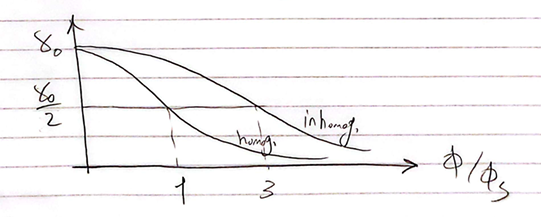
\includegraphics[scale=1]{5.png}
\end{center}
\textbf{Remarks:}
\begin{itemize}
    \item The gain also saturates but with a smaller rate; we reach half the gain at $\phi = 3 \phi_s$.
    \item We can say that we can input a larger signal before the gain saturates in inhomogenously broadened medium, but it is not necessarily the case since $\phi_s$ can be smaller from the homogeneously broadened medium.
\end{itemize}

\end{document}